\documentclass[10pt,twocolumn,letterpaper]{article}

\usepackage{cvpr}
\usepackage{times}
\usepackage{epsfig}
\usepackage{graphicx}
\usepackage{amsmath}
\usepackage{amssymb}
\usepackage{lipsum}

\graphicspath{ {images/} }

\usepackage{hyperref}
\usepackage{multicol,caption}
\newenvironment{Figure}
  {\par\medskip\noindent\minipage{\linewidth}}
  {\endminipage\par\medskip}

\usepackage[breaklinks=true,bookmarks=false]{hyperref}

\cvprfinalcopy

\def\cvprPaperID{1S3tlvllDQEO5pcDnwqr} % *** Enter the CVPR Paper ID here
\def\httilde{\mbox{\tt\raisebox{-.5ex}{\symbol{126}}}}

% Pages are numbered in submission mode, and unnumbered in camera-ready
%\ifcvprfinal\pagestyle{empty}\fi
\begin{document}

%%%%%%%%% TITLE
\title{Simulating Raindrops on a Glass Pane}

\author{Budmonde Duinkharjav\\
Massachusetts Institute of Technology\\
77 Massachusetts Ave, Cambridge, MA 02139\\
{\tt\small budmonde@mit.edu}
% For a paper whose authors are all at the same institution,
% omit the following lines up until the closing ``}''.
% Additional authors and addresses can be added with ``\and'',
% just like the second author.
% To save space, use either the email address or home page, not both
\and
Danny Tang\\
Massachusetts Institute of Technology\\
77 Massachusetts Ave, Cambridge MA 02139\\
{\tt\small data1013@mit.edu}
}

\maketitle
%\thispagestyle{empty}


%%%%%%%%% ABSTRACT
\begin{abstract}
    The simulation of liquids flowing down various types of materials has a variety of use cases across many applications of computer graphics. In this paper, we implement one of these common use cases - raindrops flowing down a glass pane. To do so, we very closely followed the work presented in a paper by Chen et al. This paper details a heuristic approach to achieving realistic, believable raindrop behavior using a variety of techniques based on observed droplet properties in real raindrops. After rendering our results with Mitsuba Physically Based Renderer, we were able to produce a video that showcases pretty realistic raindrop behavior.
\end{abstract}

%%%%%%%%% BODY TEXT
\section{Introduction}
\subsection{Motivation}
We initially decided to pursue this project because we wanted to create something simple that had a wide range of uses. We originally planned to implement a system that could simulate a variety of liquids on multiple types of materials based on user given specifications, but realized that we needed to decrease the scope of the project given our time constraints. So, we set out to simulate one type of liquid. Rain (water flowing down glass) seemed to be a natural choice, both because virtually everyone is well accustomed to how rain looks and because it is aesthetically pleasing. We were also both very interested in the particle system and rendering portions of 6.837, and this project would be a great way to combine the two. Furthermore, this project would give us experience in figuring out implementation details from a mostly abstract paper.

\subsection{Tools and Resources}

For the work presented in this paper, we used the following tools and resources:

\begin{enumerate}
    \item Chen et al's "A heuristic approach to the simulation of water drops and flows on glass panes" \cite{paper}
    \item 6.837's (Computer Graphics) particle system assignment code
    \item 6.865's (Digital and Computational Photography) image manipulation helper classes
    \item Mitsuba Physically Based Renderer \cite{Mitsuba}
    \item Vegas Pro Studio
\end{enumerate}

Our system's implementation is based closely on the heuristic techniques described in Chen et al's paper. We adapted code from 6.837 and 6.865 to set up the foundation that we would build upon. To render our results, we used Mitsuba Physically Based Renderer to produce rendered frames and Vegas Pro Studio to stitch the frames together into a video.

\subsection{Pipeline Outline}

A rough overview of our project's pipeline is as follows:

\begin{enumerate}
    \item Simulate a water droplet particle system on a 2D plane
    \item Render height maps of water on the 2D plane from each of the particle system's timesteps
    \item Render each height map using Mitsuba Physically Based Renderer
    \item Stitch the rendered height map frames together with Vegas Pro Studio
\end{enumerate}

In the first step, we run calculations to determine how our water particles move based on various properties. In the second step, we generate height maps of the water to represent how much water there is at each point in a 2D grid. In the third and fourth steps, we render frames from the generated height maps and combine them to produce a video.


%------------------------------------------------------------------------
\section{The Raindrop Particle System}

To begin, we designed a particle system to model the behavior of raindrops on a continuous 2D plane. We created two classes on top of the particle system assignment's code to represent individual rain droplets and the glass pane: $droplet$ and $windowsystem$. $Droplet$ contains properties of individual droplets such as an id and mass, and $windowsystem$ contains environmental properties such as the probability of droplets appearing on the plane.

\subsection{Particle Movement Heuristics}

To determine how droplets move within our particle system, we employed a few heuristic methods to model how real droplets move. Specifically, we tried to capture the effects of surface tension, gravity, and friction. Since surface tension is a complicated force to model, both physically and computationally, we determine the direction of movement and the speed of a droplet separately.

To calculate the direction of movement of droplets, we modeled two real life properties. The first is that water tends to move towards water that is near it, and the second is that different regions of a surface may have different affinities for water. To deal with the first, we use a height map (described in further detail in a later section) that tells us how much water is at each location of our plane. If a moving droplet has water below it, we simply have it move to the place with the most water. If a moving droplet has no water below it, then we have to deal with the second property. For this case, we use precomputed, uniformly sampled probabilities for each cell in our height map. These probabilities represent the surface's $local\ water\ affinities$, and are used to calculate which direction the droplet should go. 

To calculate the speed of movement, we calculate the sum of external forces (gravity and friction) that act upon a droplet. The acceleration of a droplet is calculated as:

\begin{equation}
    f_{ext} = f_{gravity} +f_{friction}.
\end{equation}

Gravity is evaluated as $mg$ where $m$ is the mass of a droplet and $g$ is the gravitational acceleration constant. The frictional force is modelled as a force with two modes: static friction $f_{static} = -min(m, m_{static}) g$ and kinetic friction $f_{kinetic} = -m_{static} g$. The static friction is applied to the droplet if the droplet's speed is zero; otherwise, the kinetic friction is applied.

Equation (1) tells us that for a droplet, if $m < m_{static}$ for some global $m_{static}$, the droplet will either stay still if it is not moving or will grind to a halt if it is. Meanwhile, droplets with $m > m_{static}$ will accelerate downwards. To induce initial movement and to provide realism, we randomly generate droplets of random mass on our plane at each time step.


\subsection{Residual Droplet Generation}

An interesting behavior of water flows (moving droplets) is that they leave behind residual water droplets that do not move. We implement this as a pseudo Poisson Process. First, for each moving droplet, we keep track of a time, $t$, that tells us the number of time steps it has been since the droplet last left a residual droplet. Then, at each time step, for each water flow we calculate a probability that grows with $t$, to determine whether or not a residual droplet is left. We have a value $t_{max}$ where the probability becomes 1. When a droplet leaves behind a residual droplet, we reset its $t$ to 0, and leave behind a droplet of mass $m_{residual} = min(m_{static}, \alpha m_{parent})$, where $\alpha$ is a random number between 0.1 and 0.3. Finally we substract $m_{residual}$ from $m_{parent}$.

\begin{Figure}
    \centering
    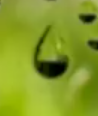
\includegraphics[width=100pt]{before.png}
    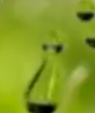
\includegraphics[width=100pt]{after.png}
    \captionof{figure}{Generation of a residual droplet.}
    \label{fig:residual}
\end{Figure}

\subsection{Water Droplet Merging}

When droplets come into contact with each other, they merge. To determine whether or not droplets should merge, we use an ID map. The ID map is a grid of a certain resolution (in our final implementation we used 1000 x 1000) that is overlayed on top of our particle system's plane. Each cell of the ID map contains a value: -1 if there is no droplet occupying that cell, and the ID of the droplet if there is. At each time step, we merge droplets if their IDs ever become adjacent to each other. If both of the merged droplets are moving, we take a weighted average of their velocities, $(m_{1}v_{1} + m_{2}v_{2})/(m_{1} + m_{2})$, and scale it with a $\mu > 1$; the scaling is done since in reality, the new water droplet tends to move faster than the two merged ones.

%-------------------------------------------------------------------------
\section{The Height Map}

Using the positions of droplets in our particle system, we can draw a \emph{height map} of the droplets in our frame. The height map is similar to the ID map; it is a grid with the same resolution as the ID map that is also overlayed on top of our particle system's plane. Construction of the \emph{height map} is done with the following three step process:

\begin{enumerate}
    \item Construct an initial \emph{height map} of a frame's droplet positions
    \item Apply a box blur to the resultant \emph{height map} to smooth out the shape of rain drops
    \item Apply an erosion operation on the \emph{height map} to simulate water trickles in a stream
\end{enumerate}

\subsection{Height Map Construction}

Each droplet in the particle system is represented in the initial height map as a collection of 1-5 (chosen at random) overlapping hemispheres. The first hemisphere's center is at the droplet's position in the particle system and each subsequent hemisphere is at a small random offset from the previous one. This allows us to create interesting water droplets that have different shapes.

\begin{Figure}
    \centering
    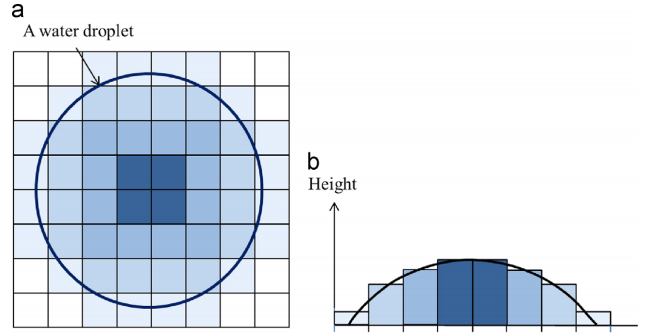
\includegraphics[width=250pt]{height.png}
    \captionof{figure}{Height of grid cells around a hemisphere.}
    \label{fig:heightdiag}
\end{Figure}

To determine the values in the height map, we use the masses of our droplets to calculate the radius of our hemispheres. A hemisphere of mass $m$ at position $p_c$ will have a radius proportional to $\sqrt[3]{r}$ with height values of nearby grid cells equal to $\sqrt{r^2 - ||p - p_c||^2}$ (Note: if $r<||p-p_c||$ the height value would be 0). At each time step, we only update the value of a cell in our existing height map if the new value is greater than the existing one.

\subsection{Blur and Erosion}

We apply a box blur with a kernel size of 3 in order to smooth out the \emph{height map} so that our combined hemispheres look more like natural droplets. We also clamp height values below a certain $\epsilon$ to 0 to prevent the whole map from filling with small values.

\begin{Figure}
    \centering
    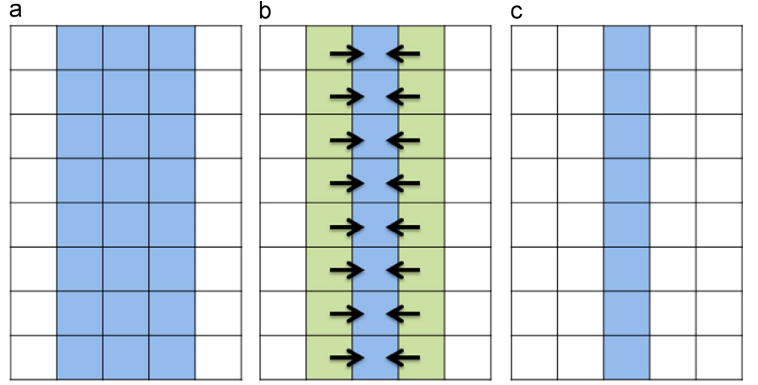
\includegraphics[width=250pt]{erosion.png}
    \captionof{figure}{Erosion affects wet cells with neighboring dry cells by moving all its water content away from the dry edge.}
    \label{fig:erosion}
\end{Figure}

We also perform an erosion operation to simulate the effect of water trickling down a stream. We note that if the height value at a grid position $(x,y)$ is non-zero but either $(x-1,y)$ or $(x+1,y)$ is not, then that means the water in grid $(x,y)$ is either the edge of a droplet or the edge of a water stream. In this case, we move the height of cell $(x, y)$ away from the edge horizontally as in figure \ref{fig:erosion}.

\begin{Figure}
    \centering
    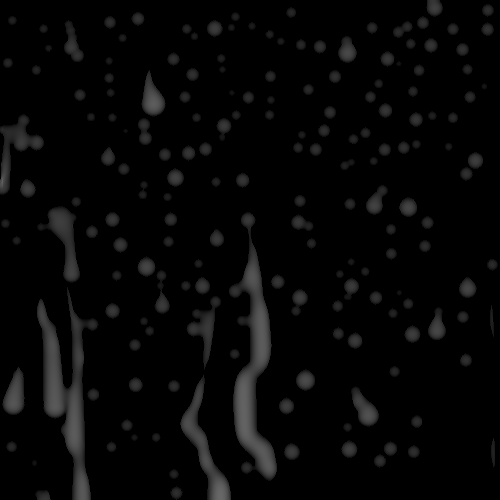
\includegraphics[width=250pt]{heightmap3553.png}
    \captionof{figure}{Height map of a frame of droplets.}
    \label{fig:heightmap}
\end{Figure}


%-------------------------------------------------------------------------
\section{Rendering}

After calculating the height maps of our particle system at each time step, we save them as grayscaled PNGs, where black corresponds to the lowest height (0) and white corresponds to the highest height. We then pass these PNGs to a renderer to produce realistic looking raindrops.

\subsection{Mitsuba}

For rendering, we used Mitsuba Physically Based Renderer. As its name suggests, Mitsuba uses physically based techniques to render scenes. We first set up a common scene that we would use to render all of our PNGs in. This included a common background, which doubled as a light source - instead of creating an explicit emitter of light such as a sphere, we used an environment map, which is a feature provided by Mitsuba that allows us to convert an image into an emitter of light based on how "radiant" its pixels are. This allowed us to achieve realistic, natural lighting with a real background. We also set up a bidirectional scattering distribution function (BSDF) to create realistic looking raindrops; we used a dielectric material for our droplets with an internal index of refraction of water (1.33) and an external index of refraction of air (1.00). Finally, we decided to use ray tracing to render our scene.

To render all of our height maps, we wrote a script to read in all of the height map PNGs and process them. For each height map, we used Mitsuba's $heightfield$ shape type to produce a 3D representation of it, where the $z$ value of the 3D representation corresponds to the pixel values in the PNG. The 3D representation becomes an actual object in the scene that we eventually render. Finally, we attach the BSDF defined before to the new object in the scene, and render it. The result is a frame with pretty realistic looking rain drops. For our final result, we rendered 3553 frames at a rate of about 2 frames per second.

\begin{Figure}
    \centering
    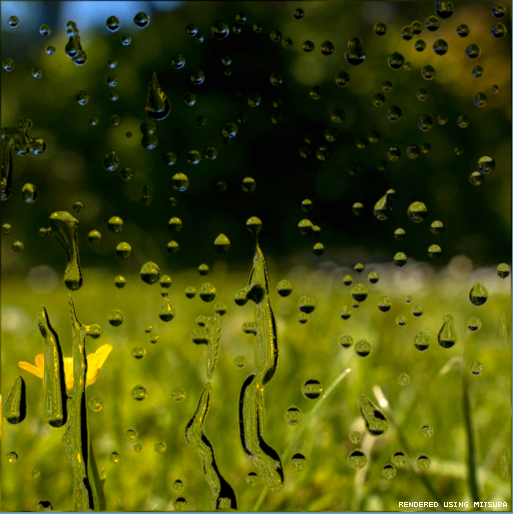
\includegraphics[width=250pt]{rendered3553.PNG}
    \captionof{figure}{Corresponding rendered frame from the height map in Figure \ref{fig:heightmap}}
    \label{fig:render}
\end{Figure}

\subsection{Sony Vegas Pro}

With Mitsuba, we rendered a separate frame for each of our generated height maps. In order to combine the frames into a video, we used Sony Vegas Pro to stitch the frames together. For our final video, we used 60 frames per second with 3553 height map PNGs to create a video that was about a minute long.


%------------------------------------------------------------------------
\section{Evaluation}

Our final video displays a pretty realistic simulation of a liquid flowing down a surface (\url{https://youtu.be/vxd8Brt67xI}). We were able to successfully capture many of the properties of liquid flows that we wanted to, such as:

\begin{enumerate}
    \item Various factors involved in droplet movements (friction, surface tension, gravity, and water affinity)
    \item Residual droplet generation
    \item Water droplet merging
\end{enumerate}

While we are pretty satisfied with our final result, we note that there are still some areas that could be improved. Firstly, the consistency of our droplets in the video feels more like oil, rather than water. This is related to the values of the parameters that we mostly arbitrarily picked for each feature that we added. Due to limitations in the speed of our system in the face of our project deadline, we were not able to really tweak these parameters much; however, we imagine that we could make our system a lot more realistic by just changing these parameters.

Secondly, due to an implementation bug on how we calculated acceleration for very small droplets, some droplets appear to be oscillating left and right as they move downwards. This is only noticeable if you pay very close attention to the video, so for our final result we determined that it was not a problem that we should prioritize.

Thirdly, we would like to improve on the performance of our system. Each of our height maps takes around 0.2 seconds to create when we have a lot of particles, and each height map takes upwards of 2 seconds to render using Mitsuba. This is drastically slower than Chen et al's original implementation, which ran in real time.

%------------------------------------------------------------------------
\section{Conclusion}

Overall, we produced a result that feels like real liquid on a surface. We were impressed by how well heuristic methods could resemble real life behaviors, especially in how we were able to model droplet movements. We were able to achieve much of what we had set out to do in our original motivation: we were able to simulate one type of liquid, were able to combine particle systems and rendering, and were able to figure out implementation details from a mostly abstract paper. At the same time, we also have a lot of room for improvement in many areas, including realism, implementation, and performance. This project has been an incredible learning experience, and has allowed us to better understand the vast world of computer graphics.

{\small
\bibliographystyle{ieee}
\bibliography{egbib}
}

\end{document}
